\documentclass[11pt, oneside]{article}   	% use "amsart" instead of "article" for AMSLaTeX format
\usepackage{geometry}                		% See geometry.pdf to learn the layout options. There are lots.
\usepackage{hyperref}  % TODO: see page 94 of latex book
\geometry{letterpaper}                   		% ... or a4paper or a5paper or ... 
%\usepackage[parfill]{parskip}    		% Activate to begin paragraphs with an empty line rather than an indent
\usepackage{graphicx}				% Use pdf, png, jpg, or eps§ with pdflatex; use eps in DVI mode
								% TeX will automatically convert eps --> pdf in pdflatex		
\usepackage{amssymb}

\title{CSCI E-181 Spring 2014 Practical 1}
\author{David Wihl\\
     \texttt{davidwihl@gmail.com}}
%\date{}							% Activate to display a given date or no date

\begin{document}
\maketitle
\section*{Warm-Up}

%\subsection*{Basic K-Means}

\par As a warmup, I synthesized five clusters of data.  I then used a K-Means implementation in Octave I had written for a previous course.\footnote{Machine Learning, Coursera, Prof. Andrew Ng, Completed Jan 2014, \url{https://class.coursera.org/ml-004}} While this implementation was sufficient for the prior course's provided dataset, when I tested it the synthesized data set, K=5 and random initial centroids, one of the centroids would frequently not converge on any points.

\begin{figure}[h!] % consider removing ! to  improve formatting and put back in subsection
\centering
\includegraphics[scale=0.6]{randominitialClusters}
\caption{Random Initial Centroids After 1 Iteration}
\end{figure}

I subsequently modified the code to use K-Medoids, choosing one of the sample data points at random as an initial centroid. This worked much better.

\begin{figure}[h!]
\centering
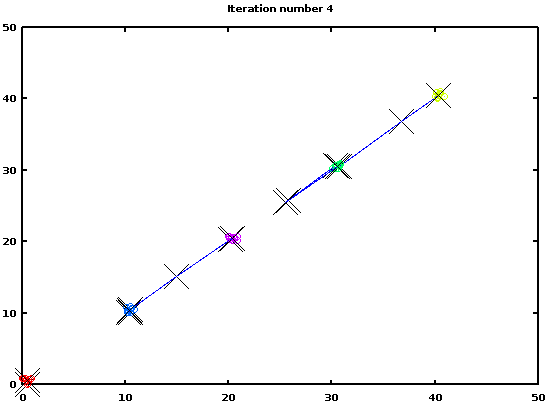
\includegraphics[scale=0.6]{K-Medoid}
\caption{K-Medoids Converge After 4 Iterations}
\end{figure}

\subsection*{CIFAR-10 Image Data}

I then attempted using K-Medoids with the CIFAR-10 Image Data, using the Matlab version of the data with Octave. The training data consists of a 10000x3072 matrix of UInt8. Each row is a 32x32x3 (=3072) color image, consisting of 1024 red, 1024 green and 1024 blue elements. There are 10 classes in the set (``airplane'', ``automobile'', etc.), so setting K=10 was a rational first step.

Percentage Distribution of K values after normalization and 10 iterations

06
05
04
26
14
13
05
04
03
15




\end{document}  
